\section{Estado del Arte}\label{sec:estado_del_arte}

Las mónadas de \textsf{Haskell} utilizan la \textit{do-notation} para facilitar la lectura y escritura de código. Posteriormente, al compilar el programa, el compilador extrae la azúcar sintáctica y remplaza la declaración de las expresiones monádicas por la evaluación de funciones $\lambda$, estas se ejecutarán de forma secuencial debido a la propia definición del operador \textit{bind}, asociada a cada mónada específica. 

Dado lo anterior, implementar la paralelización de las expresiones monádicas dentro de la \textit{do-notation} no es algo trivial de resolver. Como consecuencia del interés general de solucionar el problema anterior, este ya ha sido abordado anteriormente, por Marlow, Jones, Kmett y Mokhov en 2016, cuya solución propuesta consiste en transformar el código fuente secuencial de una mónada en una representación intermedia paralelizable, mediante el uso de functores aplicativos. De esta manera, se modifica la sintaxis y se mantiene la semántica del programa \cite{MarlowPJKM2016}. En dicho trabajo, se plantea la transformación para una mónada arbitraria; es decir, esta puede contener dependencias entre declaraciones de argumentos.

\subsection{Pipeline de transformación de do-notation: Rearrangement y Desugaring}\label{sec:sa}

El algoritmo presentado por Marlow, Jones, Kmett y Mokhov en 2016 consiste en un \textit{pipeline} de dos etapas,  \textit{rearrangement} y \textit{desugaring} \cite[p.~96]{MarlowPJKM2016}. Cada etapa comprende múltiples pasos; sin embargo, nos centraremos principalmente en la fase de \textit{rearrangement}, ya que en esta se genera el plan de ejecución óptimo para la paralelización de las expresiones monádicas. Estás últimas serán denominadas \textit{statements} de la \textit{do-notation} de aquí en adelante.

En términos de implementación y reproducibilidad, resulta especialmente relevante que esta transformación no solo exista como propuesta académica, sino que se encuentre incorporada y documentada en el compilador \textit{Glasgow Haskell Compiler} (\textsf{GHC}) como la extensión \texttt{ApplicativeDo} \cite{marlow_ado}. En particular, la documentación oficial de \textsf{GHC} describe explícitamente el propósito de la extensión: reescribir bloques do utilizando operadores aplicativos (\texttt{<\$>}, \texttt{<*>}) y, cuando corresponde, el operador \texttt{join}, de modo de maximizar el uso de una estructura de efectos estática ``tanto como sea posible'' sin alterar la semántica del programa \cite{MarlowPJKM2016}.

Esta especificación es importante para el estado del arte por dos razones: primero, porque fija un contrato público (respaldado por el compilador) respecto del comportamiento esperado de la transformación (qué formas de \texttt{do} pueden ``desazucararse'' a aplicaciones paralelizables y bajo qué limitaciones); y segundo, porque permite que cualquier propuesta de mejora (como la que plantea esta memoria) se formule en continuidad con una base establecida y validada por la comunidad, con un punto de comparación claro tanto a nivel de semántica como de comportamiento del compilador. En consecuencia, el hecho de que \texttt{ApplicativeDo} esté normada en el manual de \textsf{GHC} transforma el problema desde una idea puramente conceptual a una línea de trabajo verificable sobre una herramienta real, con pruebas y casos de uso existentes, lo que refuerza la factibilidad técnica de extender el pipeline descrito por Marlow et al \cite{MarlowPJKM2016}.

\subsubsection{Etapa de Rearrangement}\label{sec:sa}

En primer lugar, sea una expresión monádica arbitraria, la cual usa la \textit{do-notation}. En ella, se declaran múltiples \textit{statements} de la forma \verb|pi <- ei|, estos últimos se denotarán \verb|si|, donde \verb|i| es el indice asociado a cada uno de ellos. Posteriormente, este fragmento de código se transformará en un elemento de la sintaxis abstracta \verb|do l e|, donde \verb|l| es la lista de \textit{statements} \verb|{s1; ...; sn}|. 

Una vez que la expresión \verb|do| ha sido transformada en un elemento de la sintaxis abstracta, el conjunto de \textit{statements} \verb|l| se introduce como entrada al proceso de \textit{rearrangement}, el cual no considera la expresión \verb|e| dentro de sus cálculos. Este proceso tiene la siguiente descripción, desarrollada por Marlow y los otros autores antes mencionados:

\begin{figure}[ht]
    \centering
    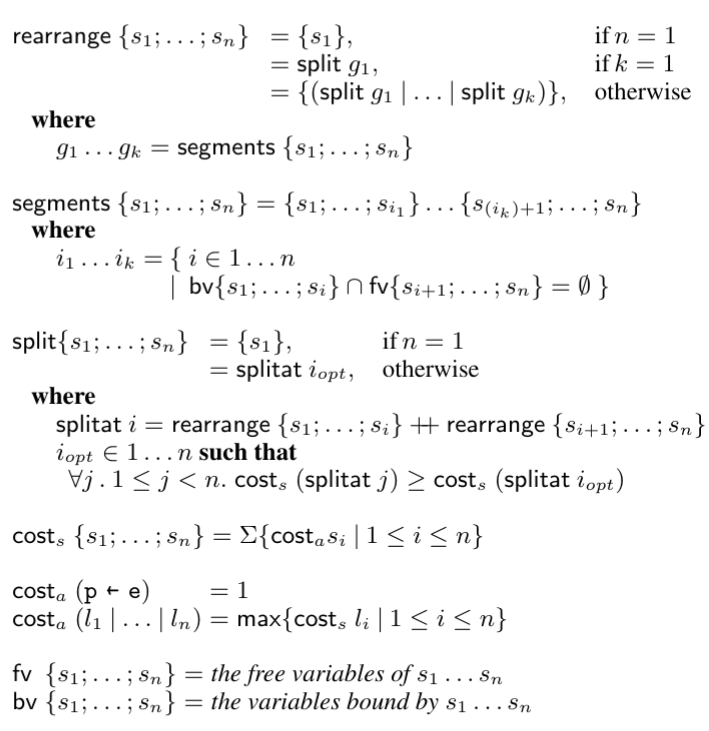
\includegraphics[width=0.51\textwidth]{imagenes/rearrangement.png}
    \caption{Proceso de \textit{Rearrangement}}
    \label{fig:mi-figura}
\end{figure}

\FloatBarrier

El proceso ya mencionado \textit{rearrangement} se encarga de generar un plan de ejecución óptimo, asociado a la cadena de \textit{statements} \verb|{s1; ...; sn}|, determinando qué segmentos se pueden paralelizar y cuáles no. La función principal de este proceso toma como nombre \verb|rearrange|. Esta última, en primera instancia, realiza un barrido secuencial de \verb|{s1; ...; sn}| para identificar los segmentos paralelizables de manera inmediata, utilizando e invocando la función \verb|segments|.

Continuando con lo anterior, la función \verb|segments| iterará sobre las posibles separaciones entre los \textit{statements}. En otras palabras, dado un conjunto de \verb|n| \textit{statements}, se consideran las \verb|n-1| separaciones posibles. Para cada separación \verb|i|, se verifica si la intersección entre el conjunto de variables definidas en \verb|{s1; ...; si}| y el conjunto de variables libres en \verb|{si+1, ..., sn}| es vacía. De ser así, se puede realizar un corte en \verb|i|, ya que no existen dependencias entre ambos grupos de \textit{statements}. Por el contrario, si la intersección no es vacía, se descarta el corte en \verb|i| debido a las dependencias existentes.

Al verificar si la intersección es vacía en la función \verb|segments|, se hace referencia a la propiedad \textit{def-use}. Esta propiedad establece que, para utilizar una variable \verb|x|, es necesario que haya sido definida previamente. Por lo tanto, si se realizara un corte en una posición \verb|i| de la lista de \textit{statements} donde la intersección no es vacía, esto indicaría que la secuencia \verb|{s(i+1); ...; sn}| hace \textit{uso} de una variable \textit{definida} en \verb|{s1; ...; si}|. En consecuencia, al realizar el corte se violaría la propiedad \textit{def-use}.

En el siguiente paso se emplea la función \verb|split|, que itera de manera similar sobre las separaciones de los \textit{statements} \verb|{s1; ...; sn}|, pero en este caso aplica \verb|rearrange| por separado a cada par de subconjuntos. Una vez obtenidas todas las combinaciones posibles, selecciona la de menor costo. 

Dado lo anterior, es necesario describir el modelo de costos utilizado por este algoritmo y la notación para representar ejecuciones paralelas de \textit{statements}. Para estas últimas, dado un conjunto \verb|{l1, ..., ln}| de secuencias de \textit{statements} que pueden ejecutarse en paralelo, se utilizará en la sintaxis abstracta la notación \verb!(l1|...|ln)!. En concecuencia, el modelo de costos se define de la siguiente manera:

\begin{verbatim}
    cost(p <- e)        = 1
    cost({s1; ...; sn}) = sum { cost(si) | i in {1, ..., n}}
    cost(l1|...|ln)     = max { cost(li) | i in {1, ..., n}}
\end{verbatim}

Se observa que, el costo de una secuencia de \textit{statements} no paralelizables corresponde a la suma de los costos individuales de cada \textit{statement}. Por otra parte, para un conjunto de secuencias que pueden ejecutarse en paralelo, el costo total será el máximo valor entre los costos de cada secuencia. Finalmente, en el caso unitario de un solo \textit{statement}, el costo será igual a 1.

Finalmente, como se mencionó antes, la función \verb|split| selecciona el plan de ejecución óptimo con el costo mínimo, cuya acción resulta computacionalmente cara debido a las múltiples llamadas recursivas. Posteriormente, luego de producir el nuevo orden de ejecución, este se guarda en el elemento \verb|l'| de la sintaxis abstracta, siendo retornado el objeto \verb|do l' e| para su futuro procesamiento en la etapa de \textit{desugaring} 


\subsubsection{Etapa de Desugaring}\label{sec:sa}

La siguiente etapa corresponde al proceso de \textit{desugaring}, que aplica \textit{pattern matching} recursivo sobre el objeto retornado por la etapa de \textit{rearrangement} \verb|do l' e|. Los casos que abarca esta etapa se describen en la siguiente figura:

\begin{figure}[ht]
    \centering
    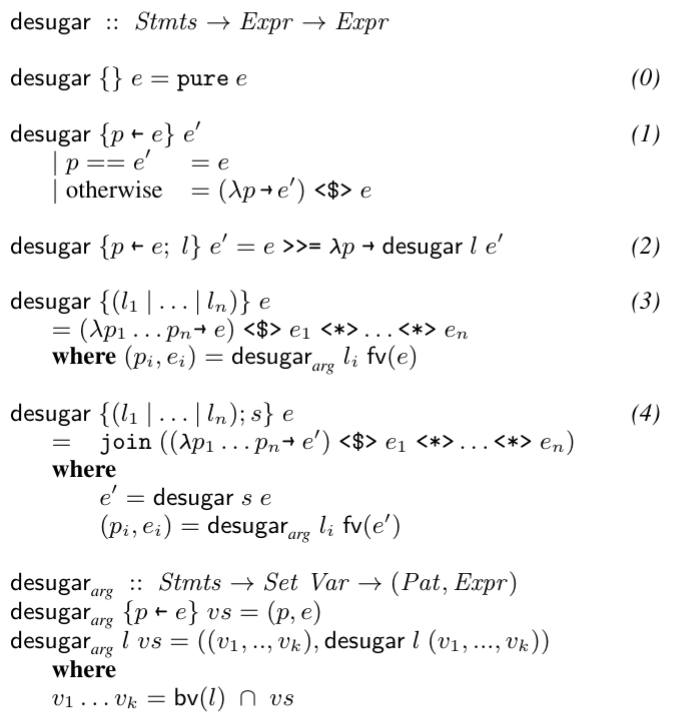
\includegraphics[width=0.51\textwidth]{imagenes/desugar.png}
    \caption{Proceso de \textit{Desugaring}}
    \label{fig:mi-figura}
\end{figure}

Se observa que, la función \verb|desugar| considera cada escenario posible dentro del \textit{pattern matching}. Este último, se ejecuta sobre la lista de \textit{statements} \verb|l'| que fue generada en el proceso de \textit{rearrangement} de forma previa. Continuando con la descripción de esta función, dependiendo del caso, se usarán los operadores asociados a \textit{functores aplicativos} o a su subclase, las \textit{mónadas}. 

\FloatBarrier

\subsubsection{Aplicación del algoritmo}\label{sec:sa}

Para ilustrar el flujo del algoritmo descrito, se ingresará como entrada el ejemplo mostrado en la sección \ref{sec:intro}, aquel que modela el lanzamiento de dos dados, cuya cantidad de caras es determinada por dos lanzamientos previos. Por tanto, el código asociado es el siguiente:

\begin{verbatim}
    do
        d1 <- uniform [1 .. 6]
        d2 <- uniform [1 .. 6]
        d3 <- uniform [1 .. d1]
        d4 <- uniform [1 .. d2]
        return (d3, d4)
\end{verbatim}

En primer lugar, este fragmento de código debe ser transformado a un elemento de la sintaxis abstracta de la forma \verb|do l e|. Este último, tendría la siguiente estructura:

\begin{verbatim}
    do
        {d1 <- uniform [1 .. 6];
        d2 <- uniform [1 .. 6];
        d3 <- uniform [1 .. d1];
        d4 <- uniform [1 .. d2]} (d3, d4)
\end{verbatim}

Continuando con el algoritmo, la lista de \textit{statements} debe ser transformada por el proceso de \textit{rearrangement}. Este mismo, ejecuta \verb|segments| sobre \verb|l|, identificando tres posibles puntos de corte. Sin embargo, ninguno de ellos resulta viable debido a las dependencias existentes. Por consiguiente, la función retorna \verb|l| sin modificaciones.

En el siguiente fase, se aplica la función \verb|split| sobre \verb|l|. En donde los posibles valores de corte son \verb|{1, 2, 3}|. Para simplificar la notación, se definirán las siguientes equivalencias: 

\begin{verbatim}
    s1 = d1 <- uniform [1 .. 6]
    s2 = d2 <- uniform [1 .. 6]
    s3 = d3 <- uniform [1 .. d1]
    s4 = d4 <- uniform [1 .. d2]
\end{verbatim}

Dada la notación anterior, las combinaciones posibles que son generadas por la función \verb|split|, y que posteriormente solo se escogerá la óptima con menor costo, son:

\begin{verbatim}
    i = 1 -> {rearrange s1; rearrange {s2; s3; s4}}
    i = 2 -> {rearrange {s1; s2}; rearrange {s3; s4}}
    i = 3 -> {rearrange {s1; s2; s3}; rearrange s4}
\end{verbatim}

Ignoremos las llamadas recursivas a la función \verb|rearrange| y consideremos solo lo que retornan, de esta forma obtenemos los siguientes costos asociados a cada plan de ejecución posible:

\begin{verbatim}
    i = 1 -> {s1; s2; (s3|s4)}  -> cost() = 3
    i = 2 -> {(s1|s2); (s3|s4)} -> cost() = 2
    i = 3 -> {(s1|s2); s3; s4}  -> cost() = 3
\end{verbatim}

En este punto, es evidente cuál opción debe seleccionar la función \verb|split|: la segunda opción, con un costo igual a 2. Con ello, la llamada principal a \verb|rearrange| finaliza y se retorna el plan de ejecución \verb!{(s1|s2); (s3|s4)}! en el objeto \verb|do l' e| de la sintaxis abstracta, obteniendo como resultado:

\begin{verbatim}
    do {(d1 <- uniform [1 .. 6] | d2 <- uniform [1 .. 6]);
        (d3 <- uniform [1 .. d1] | d4 <- uniform [1 .. d2])} (d3, d4) 
\end{verbatim}

En la siguiente etapa, el elemento anterior es dado como entrada a la función \verb|desugar|, la cual retornará el códifo final:

\begin{verbatim}
    join ((\d1 d2 ->
        (\d3 d4 -> (d3, d4) <$> uniform [1 .. d1] <*> uniform [1 .. d2])) 
            <$> uniform [1 .. 6] <*> uniform [1 .. 6])
\end{verbatim}

No obstante, el plan de ejecución retornado por la etapa de \textit{rearrangement} no es el óptimo para nuestro ejemplo, ya que \verb|s3| no necesita esperar a \verb|s2|, lo que si se está haciendo; lo mismo sucede con \verb|s4| y \verb|s1|. 

Lo ideal para nuestro ejemplo sería disponer de dos sub-bloques de cómputo dentro de la notación monádica, de modo que el plan de ejecución óptimo fuera \verb!{{s1; s3}|{s2; s4}}!. A primera vista, podría parecer que tiene el mismo costo igual a 2. Sin embargo, si modificamos los costos de \verb|s1| y \verb|s4| a 2 unidades cada uno, se observa que el plan de ejecución generado por el algoritmo actual \verb!{(s1|s2); (s3|s4)}! tendría un costo de 4, mientras que el óptimo \verb!{{s1; s3}|{s2; s4}}! tendría un costo de 3.

\subsection{Mónadas conmutativas}\label{sec:sa}

En el caso general, los \textit{statements} dentro de la \textit{do-notation} no pueden reordenarse porque esto alteraría la semántica del programa. Sin embargo, para una subclase particular de mónadas; llamadas \textit{mónadas conmutativas}, este reordenamiento sí es posible sin afectar la semántica del programa. Esta situación se refleja en el ejemplo del lanzamiento de una moneda y un dado presentado en la Sección \ref{sec:intro}:

\begin{tabular}{ccc}
    \begin{minipage}{0.4\textwidth}
        \begin{verbatim}
flipCoinRollDice = do 
    c <- uniform [Head, Tail]
    d <- uniform [1 .. 6]
    return (c, d)
        \end{verbatim}
    \end{minipage}
    &
    \Large $\Leftrightarrow$
    &
    \begin{minipage}{0.3\textwidth}
        \begin{verbatim}
flipCoinRollDice = do 
    d <- uniform [1 .. 6]
    c <- uniform [Head, Tail]
    return (c, d)
        \end{verbatim}
    \end{minipage}
\end{tabular}

Si bien este puede parecer un ejemplo simple, da a entender que la declaración de una expresión monádica mediante la \textit{do-notation}, en el caso de las mónadas conmutativas, puede tener distintas sintaxis que preservan la misma semántica. Esta equivalencia semántica solo es posible cuando se presentan \textit{statements} unitarios independientes o subconjuntos de \textit{statements} que son mutuamente independientes.

%%%%%%%%%%%%%%%%%%%%%%%%%%%%%%%%%%%%%%%%%%%%%%%%%%%%%%%
Este tipo de mónadas no son consideradas en el algoritmo presentado por Marlow et al., ya que el pipeline de \texttt{ApplicativeDo} está diseñado deliberadamente para no reordenar el conjunto de statements: la función \texttt{rearrange} se limita a agrupar y particionar la secuencia de declaraciones, preservando el orden relativo original. En términos operacionales, esto se manifiesta en que, incluso si el plan de ejecución resultante se representa como un árbol (con secuencias y paralelismos), al ``aplanar'' dicha representación se recupera nuevamente la lista de \textit{statements} en el mismo orden en que aparecían en el \texttt{do} original \cite[p.~95]{MarlowPJKM2016}.

Esta decisión de diseño es coherente con el caso general: en una mónada arbitraria, reordenar dos declaraciones puede cambiar la semántica del programa cuando existen efectos observables o dependencias sutiles. No obstante, el propio trabajo de Marlow et al. reconoce explícitamente que existe un caso particular donde este impedimento puede levantarse: cuando la mónada satisface una noción de conmutatividad, el intercambio de subcómputos independientes puede preservar la semántica. En ese sentido, el reordenamiento aparece como un ``gap'' natural del enfoque actual: el algoritmo no lo implementa, pero su pertinencia está motivada por el mismo marco teórico del paper, quedando como una línea plausible de extensión \cite[p.~94]{MarlowPJKM2016}.

Una gran oportunidad de optimización, por tanto, consiste en incorporar reordenamientos semánticamente válidos (bajo hipótesis de conmutatividad) antes o durante el proceso de \textit{rearrangement}, con el objetivo de ampliar el espacio de planes de ejecución evaluados y, de esta forma, obtener planes con menor costo asociado bajo el modelo del artículo \cite{MarlowPJKM2016}. Esto es particularmente relevante en programas probabilísticos, donde aparecen con frecuencia subcómputos que son independientes en el sentido probabilístico (o cuasi-independientes), pero que no quedan contiguos en el orden sintáctico original y, por ende, no pueden ser separados por cortes simples sin un reordenamiento previo.

\newpage

En el ejemplo discutido, si se hubiera considerado el intercambio de los \textit{statements} \verb|s2| y \verb|s3| asociados a nuestro ejemplo de los dados, se mantendría la semántica de tal forma:

\begin{tabular}{ccc}
    \begin{minipage}{0.4\textwidth}
        \begin{verbatim}
do
    d1 <- uniform [1 .. 6]
    d2 <- uniform [1 .. 6]
    d3 <- uniform [1 .. d1]
    d4 <- uniform [1 .. d2]
    return (d3, d4)
        \end{verbatim}
    \end{minipage}
    &
    \Large $\Leftrightarrow$
    &
    \begin{minipage}{0.3\textwidth}
        \begin{verbatim}
do
    d1 <- uniform [1 .. 6]
    d3 <- uniform [1 .. d1]
    d2 <- uniform [1 .. 6]
    d4 <- uniform [1 .. d2]
    return (d3, d4)
        \end{verbatim}
    \end{minipage}
\end{tabular}

Posteriormente, al ingresar a la etapa de \textit{}{rearrangement}, durante la primera iteración de \verb|segments|. Esta habría realizado el corte directamente en \verb|i=2|, debido a que las variables definidas en \verb|{s1, s3}| son \verb|{d1, d3}|, mientras que las variables utilizadas en \verb|{s2, s4}| son únicamente \verb|{d2}|. Al calcular la intersección, esta resulta vacía, por lo que se procede con el corte. Finalmente, el plan de ejecución resultante será \verb!{{s1; s3}|{s2; s4}}!, que corresponde al óptimo esperado. Este plan generaría el siguiente código tras pasar por el proceso de \textit{desugaring}:

\begin{verbatim}
    (\d3 d4 -> (d3, d4))
        <$> (uniform [1 .. 6] >>= (\d1 -> uniform [1 .. d1]))
        <*> (uniform [1 .. 6] >>= (\d2 -> uniform [1 .. d2]))
\end{verbatim}

\new

\subsubsection{Teoría de distribuciones}

La noción de mónada conmutativa resulta particularmente natural en el contexto probabilístico porque, en una formulación estándar, el muestreo de variables aleatorias independientes es conmutativo a nivel semántico: si dos subcómputos no comparten dependencias de datos (no existe relación \textit{def-use} entre sus variables), entonces permutar su orden no altera la distribución conjunta inducida por el programa, sino únicamente el orden sintáctico en que se generan los valores. En otras palabras, el efecto probabilístico asociado a ``elegir'' un valor para una variable y luego para otra, cuando ambos efectos son independientes, puede interpretarse como un producto de distribuciones que es conmutativo. Esta intuición es precisamente la que se busca capturar cuando se afirma que las mónadas de probabilidad constituyen un caso canónico donde el reordenamiento de \textit{statements} puede preservar la semántica.

Desde un punto de vista más formal, Kock presenta una caracterización axiomática en la cual las mónadas conmutativas pueden entenderse como una teoría general de distribuciones \cite{Kock2012}. En este marco, la conmutatividad no se plantea como un ``truco'' sintáctico, sino como una propiedad algebraica que garantiza que ciertas combinaciones de efectos (por ejemplo, formar distribuciones conjuntas a partir de efectos independientes) son invariantes bajo permutación. Esto aporta una justificación teórica para tratar el caso probabilístico como un candidato privilegiado a extensiones del pipeline de \texttt{ApplicativeDo}: si se dispone de criterios para identificar independencia (p. ej., ausencia de dependencias \textit{def-use} entre subcómputos), entonces la conmutatividad permite, en principio, reordenar con seguridad esos subcómputos y exponer paralelismo que el algoritmo actual no alcanza por restringirse a particiones que respetan el orden sintáctico original.

\newpage

Complementariamente, Jacobs estudia de manera sistemática varias mónadas de probabilidad (incluyendo construcciones clásicas como la mónada de Giry y variantes relacionadas con expectativa), y discute condiciones bajo las cuales estas estructuras admiten nociones de conmutatividad relevantes para modelos probabilísticos \cite{Jacobs2018}. En términos prácticos para esta memoria, estas referencias permiten sostener la idea de que, bajo supuestos razonables (por ejemplo, muestreos independientes y ausencia de efectos observables adicionales), las mónadas de probabilidad se comportan como mónadas conmutativas, por lo que el reordenamiento de \textit{statements} independientes puede considerarse semánticamente válido. En consecuencia, el ``salto'' desde la teoría a la propuesta técnica es directo: si el compilador puede detectar independencia estructural en un bloque \texttt{do}, entonces un paso adicional de reordenamiento, justificado por conmutatividad, puede aumentar el espacio de planes de ejecución posibles y mejorar la paralelización obtenida.


%%%%%%%%%%%%%%%%%%%%%%%%%%%%%%%%%%%%%%%%%%%%%%%%%%%%%%%%%%
